\documentclass[Main]{subfiles}

\begin{document}
\chapter{Lagrangian Systems and Peierls Brackets}
   %introduzione
	\danger .. introduzione
		dedichiamo sforzo alla definizione dei sistemi lagrangiani astratti per dare un punto di vista unificato ai sistemi a gradi libertà continui (continui macroscopici, fluidi, campi) e a gradi di libertà discreti
		Li vediamo come sotto classi dei sistemi lagrangiani
		notiamo che in entrambi i casi c'è un possibile dato di cauchy
		usiamo questo ingrediente per definire l'algoritmo di peierls.
	\danger

	\section{Abstract Mechanical Systems}
	It's possible to state a mathematical definition sufficiently broad to include all the systems in ordinary analytical mechanics regardless of the cardinality of degrees of freedom  in a unified way.
	
	\begin{definition}[Abstract Evolutive System]
		Pair $(E,P )$ composed of:
		\begin{itemize}
			\item $E \xrightarrow{\pi} M$ \\smooth fiber bundle of typical fiber $Q$ on  manifold $M$ called \emph{"configuration bundle"}.
			\item	$ P : \Gamma^\infty(E) \rightarrow \Gamma^\infty(E)$ \\  operator called \emph{"motion operator"}
		\end{itemize}
	\end{definition}
	This formultation is still very distant from the physical interpretation but has the benift to highlight the minimal mathematical objects which must be fixed in order to specify a mechanical systems.
	
	
	\paragraph{Kinematics}
	%Fibrato Configurazione incompassa la cinematica
	The configuration bundle encompass all the kinematical structure of the system, the pivotal role is played by the smooth sections  which are to be understood as all the possible conformation of the system.

	\begin{notationfix}
		\begin{displaymath}
			\Conf \coloneqq \Gamma^\infty(M,E)
		\end{displaymath}
		Space of kinematic configurations.
	\end{notationfix}

	A section is not a statical configuration, equivalent to a specific point in the configuration space of ordinary classical systems, but has to be seen as a specific realization of the kinematics in the sense of  a complete description of a possible motion.
	At this level of abstraction, since no space-time structure has been specified, terms like stasis and motion must be taken with care .The natural physical interpretation should be clearly manifested through the concrete realization of systems with discrete and continuous degree of freedom.
	
	\begin{observation}[Mathematical structure]
	Mathematically speaking this set should be regarded as an infinite dimensional Manifold. 
	\\
	This framework provides a geometric characterization of the notion of variations as tangent vectors on the the space of kinematic configurations .\cite{Forger2005}
	\end{observation}
	
	\begin{observation}[Coordinate Representation]
	The choice of a chart atlas $\Atlas(M)$ on the base space $M$ and $\Atlas(E)$ on the total space $E$ provides a correspondence between each configuration $\gamma \in \Conf$ and family of smooth real functions $\{f_{\alpha \beta}:A_\alpha \subset \Real^m \rightarrow \Real^q \}$.
	The process is trivial:
	\begin{displaymath}
		\gamma \in \Conf \mapsto \{f_{A,U}=\psi_U \circ \gamma \circ \psi_A^{-1} \vert (A,\psi_A) \in \Atlas(M), (U,\psi_U)\in \Atlas(E)   \}
	\end{displaymath}
	
	%	$\forall (A,\psi_A)$ local chart on $M$ and $(U,\psi_U)$ local chart on $E$ such that $\gamma(A) \cap U \neq \emptyset$ $f_{A,U}=\psi_U \circ \gamma \circ \psi_A^{-1}$

	Since the whole section as a global object is quite difficult to handle is customary in field theory to work in the more practical local representation. 
	\end{observation}	
	
	\begin{observation}[Further specification of the system's kinematics]
	 	The general formalism doesn't require any other structure to be carried forward.
	 	Additional structure on the fiber , the base or the whole bundle are to be prescribed in order to specify a precise physical model, e.g. the spin structure on $E$ for the Dirac Field.\cite{Benini}
	 \end{observation}	
	
	\paragraph{Dynamics}
	The operator $P$ is the object that contains all the information about the dynamic evolution of the system.
	It has the role to select the dinamically compatible configuration among all the admissible kinematic configurations of $\Conf$, exactly as it happens in analytical mechanics where the dynamic equations shape the natural motions.
	\begin{notationfix}
		Provided an equations of motion operator
		\begin{displaymath}
			P: \Conf \rightarrow \Conf
		\end{displaymath}
		The space
		\begin{displaymath}
		\Sol \coloneqq \ker(P) \subset \Conf
		\end{displaymath}
		containing all the smooth solutions is called \emph{"Space of Dynamical Configurations"}.
	\end{notationfix}
	
	\begin{figure}[h!]
 	 	\caption{Geometric picture of the basic mechanical system's structure.}
 	 	\danger immagine
   		%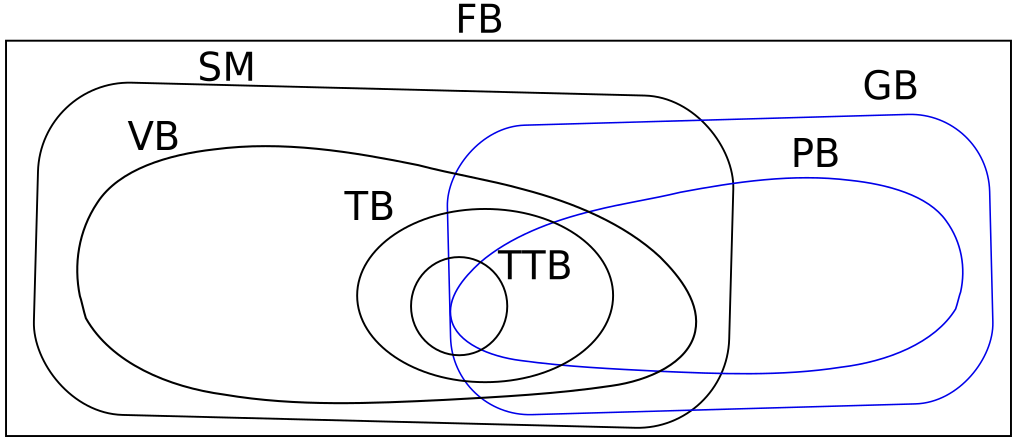
\includegraphics[width=0.5\textwidth]{Pictures/EuleroVenn_Bundles} 
  		\centering
	\end{figure}	
	
	\subsection{Lagrangian Dynamics}	
	Lagrangian systems constitute a subclass of the abstact mechanical systems of more practical interest:	
		\begin{definition}[Lagrangian System]
	Pair $(E, \mathcal{L} )$ composed of:
		\begin{itemize}
			\item $E \xrightarrow{\pi} M$ \\smooth fiber bundle of typical fiber $Q$ on the oriented manifold $(M,\mathfrak{o})$ called \emph{"configuration bundle"}.
			\item	$ \Lagrangian : J^r E \rightarrow \wedge^m T^*M$ \\bundle-morphism from the r-th Jet Bundle to  the top-dimensionial forms bundle over the base manifold $M$  called \emph{"Lagrangian density"} or simply \emph{"Lagrangian"} of r-th order.
		\end{itemize}
	\end{definition}	
	
	\begin{NB}
		IIn what follows all the systems considered will be exclusively of first order.
	\end{NB}	
	
	
	%la lagrangiana incompassa la dinamica
	In this case is the Lagrangian density the object containing all the information about the dynamic evolution of the system.

	%In Layman terms la lagrangiana  è un qualcosa che può essere integrato sopra la varietà
	In order to reconstruct the system's dynamic from the Lagrangian density has to be understood the mathematical nature of $\Lagrangian$.
	$\Lagrangian$ maps point $q_p$ on the fiber $J^r_p E$ to a m-form on $T_p M$.
	Recalling the definition of jet bundles is clear that for each smooth section on $E$ is associated a smooth section on the b$J^rE$ :
	\begin{displaymath}
		\phi \in \Gamma^\infty (E) \mapsto (\phi, \partial_\mu \phi, \partial_{\mu, \nu} \phi , \ldots \partial_{\vec{\alpha}}\phi)
	\end{displaymath}
	where  $\vec{\alpha}$ is a multi-index of length r.
	The correspondence is not univocal since sections equal up to the r-th order define the same jet section.
	The smoothness of $\Lagrangian$ ensure that each jet bundle section is mapped to a smooth section in the top-forms bundle i.e. the most general integrable object on a orientable manifold.
	
	%la classe delle densità lagrangiane
	It should be clear that $\Lagrangian$ is a specific choice among the vast class of functions suitable to be a good Lagrangian density over the  Configuration Bundle $E$:
	\begin{definition}[Lagrangian Density on the bundle $E$]
		\begin{displaymath}
			\Lag^r (E) \coloneqq \hom\biggr(J^r E,\quad \bigwedge^m( T^*M)\biggr)  \cong \big\{f:\Gamma^\infty(J^r E) \rightarrow \Omega^m(M)  \big\}
		\end{displaymath}
	(where $\Omega^m(M)$ is the common name for $\Gamma^\infty \big( \bigwedge^m( T^*M) \big)$ in the context of Grassmann algebras.)
	The equivalence states the fact that a bundle-morphism induce a mapping between the sections.
	\end{definition}
	 this choice fix the "Dynamical identity" of the considered system.
	\begin{proposition}
		$\Lag^r(E)$ has an obvious vector space structure inherited by the linear structure of $\Omega(M)$.
	\end{proposition}
	
	
	Thanks to the correspondence between a section $\phi \in \Conf$ and his r-th jet, it's possible to consider the Lagrangian as directly acting on the kinematic configurations.
	In layman terms the image  $\Lagrangian [ \phi ] \textrm{d}\mu$ , where $\textrm{d}\mu$ is the measure associated to the orientation $\mathfrak{o}$, is something that can be measured over the whole base space. 
	\\
	This property suggests the introduction of the class of associated functionals:
	\begin{definition}[Lagrangian functional]
		Is a functional on $\Conf$ with values on regular distribution over M associated to the generic $\Lagrangian \in \Lag$.	
		\begin{displaymath}
			\mathcal{O}_\Lagrangian : \Conf \rightarrow \big( C^\infty_0(M) \big)'
		\end{displaymath}			
			Such that the lagrangian functional associated to $\Lagrangian$, valued on the configuration $\phi \in \Conf$ and tested on the test-function $f \in C^\infty_0(M)$ it's given by:
		\begin{displaymath}
			\mathcal{O}_\Lagrangian [\phi] (f) = \int_M \Lagrangian [\phi] f \textrm{d}\mu
		\end{displaymath}		
	\end{definition}	
	
	\begin{proposition}
		As a distribution $\mathcal{O}_\Lagrangian [\phi] (f) $ is necessarily linear in the test-functions entry but not in the configurations entry.	
	\end{proposition}	
	
	\begin{observation}
		The choice of the image of $\mathcal{O}_\Lagrangian$ as a distribution it's a necessary precaution to ensure that functional is \emph{"convergent"} whatever is the configuration on which is evaluated.
		In fact, despite $\Lagrangian [ \phi ]$ is integrable with respect to the measure $\textrm{d}\mu$, it's not necessary summable if the support of the configuration $\phi$ becomes arbitrarily large.
		\\
		This is a simple consequence of the well known sequence of inclusions:
		\begin{displaymath}
			\Lagrangian [ \phi ] \in C^\infty_0(M) \subset L^1_{\textrm{loc}}(M,\mu) \supsetneqq  L^1(M,\mu) 
		\end{displaymath}
		of the functional analysis .
		Indeed, the functional
		\begin{displaymath}
			\mathcal{O}_\Lagrangian [\phi]= \int_{\supp(\phi)} \Lagrangian [\phi] \textrm{d}\mu
		\end{displaymath}
		is well defined for all $\Lagrangian \in \Lag^r(E)$ only over the compactly supported sections. 
		To take account of the global sections it's sufficient to dampen the integral multiplying the integrand with an arbitrary test-function.
	%il funzionale lagrangiana totale e azione
	\end{observation}
	
	\begin{notationfix}
		When calculated for the specific density of the Lagrangian system $\mathcal{O}_\Lagrangian$ takes the name of \emph{Action} or \emph{Total Lagrangian}. 
	\end{notationfix}

	The introduction of the Lagrangian density is meaningless without the prescription of a dynamical principle which allows to determine univocally a differential operator $P$ on the kinematics configurations space $\Conf$.
	This fundamental principle is the \emph{least action principle}.
	A proper justification of this claim should require the presentation of the differential calculus on the infinite dimensional manifolds $\Conf$. 
	Jumping straight to the conclusion we can state this correspondence as a principle  in term of a function which assign for all lagrangian densities an operator on the kinematic configurations space. In the case of first order lagrangian we define
	\begin{definition}[Euler-Lagrange operator]
		It's the differential operator
		\begin{displaymath}
			Q_\chi : \Conf \rightarrow \Conf
		\end{displaymath}
		relative to the lagrangian density $\chi \in \Lag^1(E)$, such that:
		\begin{equation}
			Q_\chi (\gamma) = \Biggr( \partial_\mu \biggr( \frac{\partial \chi}{\partial(\partial_\mu \phi)} \biggr\vert_\gamma \biggr) - \frac{\partial \chi}{\partial \phi}\biggr\vert_\gamma \Biggr) \qquad \forall \gamma \in \Conf
		\end{equation}
		(where 	$\biggr( \frac{\partial \chi}{\partial(\partial_\mu \phi)}$ is the be intended as the lagrangian density constructed differentiating $\chi(\phi, \partial_\mu)$ as an ordinary function treating its functional entries as an usual scalar variable.)
	\end{definition}
	\begin{observation}
		
	\end{observation}
	
	\begin{observation}
		The whole theory of both Lagrangian densities class and Euler-Lagrange equation could be stated in a more syntetic way in terms of the Grassmann-graded variational bicomplex.\cite{Giachetta2009}\cite{Sardanashvily}
	\end{observation}
	
		

	
%-_-_-_-_-_-_-_-_-_-_-_-_-_-_-_-_-_-_-_-_-_-_-_-_-_-_-_-_-_-_-_-_-_-_-_-_-_-_-_-_-_-_-_-_-_-_-_-_-_-_-_-_-_-_-_
%\newpage
	\section{Concrete Realization}
	In the previous section we claim that the abstract definition of Lagrangian systems is broad enough to encompass all the classical lagrangian systems with both discrete degrees of freedom, like particles, and continuous degree of freedom, like fluids or fields.
	Let' show two of the most significant examples.
	%esibiamo quanto è ampia la nostra definizione
	
	
	
		\subsection{Classical Linear Field over a Space-Time}
		\danger così com'è la definizione è troppo forte?	
		
		
			The field systems are a subset of the lagrangian systems:
			\begin{definition}[Linear Fields on curved Background]
				It's a Lagragian system $(E,\Lagrangian)$ such that:
				\begin{itemize}
					\item the configuration bundle $E\xrightarrow{\pi} M$ is a \underline{vector bundle}.
					\item the base manifold $M$ is a \underline{Globally Hyperbolic Spacetime}.
					\item the Euler-Lagrange operator $P= Q_\Lagrangian$ is a \underline{Green Hyperbolic operator}.
					\item For each Cauchy surface $\Sigma \subset M$ can be defined a well-posed Cauchy problem for the motion equation of $P$.\footnote{Green-hyperbolic operators are not necessarily hyperbolic in any PDE-sense and that they cannot be characterized in general by well-posedness of a Cauchy problem. \cite{Terlaky2010} \cite{Bar2010}}
				\end{itemize}
			\end{definition}
		The idea of taking bundles on a space-time manifold it's physically intuitive, kinematically speaking a fields configuration it's not more than an than an association of some element of the fiber $Q $ for each point of the space-time $M$.
		But the other three condition are worth a deeper insight:

		\paragraph{Vector Bundle Condition}
			Even if it might make sense to speak of nonlinear fields in some more general context, this condition it's a necessary element in case some form of the \emph{superposition principles} as to be taken in account.
			Obviously this hypothesis is not sufficient to formulate the principle in the strong classical way, i.e.:"the response at a given place and time caused by two or more stimuli is the sum of the responses which would have been caused by each stimulus individually" mostly because only free systems can be considered at this stage and any statement about stimulus can make sense.
			\\
			However It assure that $\Conf$ is a vector space and , in conjunction with the linearity of motion operator $P$, $\Sol= \ker(P)$ is a linear subspace.		
			In other words every linear combination of kinematic configuration it's still a kinematic configuration.

		\paragraph{Global hyperbolicity condition.}
		
			This condition is strictly connected to the dynamic behaviour of the system.
			
			\danger
			Def di dominio di dipendendenza
			footnote di definizione di spazio tempo
			def cauchy surface
			Remark causal future past
			def globally hyperbolic
			Teorema sulle caratterizzazioni
			\begin{notationfix}
				We denote the set of all the cauchy surfaces as $\PowerSet_{C}(M)$.
			\end{notationfix}
					

		Glon iperbolic determina la fogliazione dello spazio tempo per superfici di cauchy
		La superficie di cauchy è questa:
		\begin{definition}[Cauchy surface]
		\end{definition}		
		questo da la possibilità della buona posizione dei problemi di cauchy.. fisicamente è la condizione minima per definire i dati iniziali dell'evoluzione dinamica.
		definisco data...
		
	No!		La definizione di green hyperbolicity garantisce invece l'esistenza e unicità del problema di cauchy associata
		
		e non solo, anche l'esistenza degli operatori di green associati che sono ingrediente fondamentale della costruzione di peierls

		M è glob iper e P è green iper per tener conto del comporatamento propagativo
		definire sup cauchy
		definire s-t iperbolico (solo la caratterizzazione di ammetre una sup di cauchy)
		definire op green iperbolico su spazio tempo iperbolico (cioè ha delle green ope)
		Propr di buona definizione esistenza e unicita della soluzione
		
		Di particolare ricorrenza fisica sono gli operatori normally iperbolic
		espressione in coordinate
		esempio K-g!
		\danger

		
		\danger
		
		Secondo bar e ginoux per parlare di campo classico non serve specificare nient'altro...
		la condizione di $\exists  1!$ operatore di green di $P$  insieme a quella di Essere un sistema lagrangiano è un requisito minimo  per definire senza ambiguità le parentesi di peierls.
		
		la condizione di green-hyperbolicity ( che garantisce di $\exists 1!\; E^\mp$ ma non che  $\exists 1!$ soluzione del PC) corredata della scelta di un pairing permette di quantizzare secondo lo schema algebrico
		
		La condizione di well-posedness del problema di cauchy da la possibilità di quantizzare secondo lo schema dei dati iniziali
		
		in tutti questi casi la candizione di Globally -hyperbolic per lo spazio tempo sottostante è necessaria
		\danger


		\paragraph{Green-Hyperbolicity condition.}
			The third condition  ensures the existence of the Green's Operator as follows directly from definition.
			\danger \textbf{Memento:}
				Pensavo di utilizzare la definizione di Green hyperbolic data da Bar che si avvale del concetto di formally dual (che non richiede la presenza del pairing) invece di quella usata in Advances AQFT che richiede solo che ammetta almeno un $G^\pm$  per poi dimostrare tramite teorema che se è anche autoaggiunto vale l'unicità. Si tratta solo di una piccola sfumatura.. Deve essere chiarito che in tutto ciò che faccio interessano che $$\forall P \, \exists1!G^\pm$$.
				Che poi questa condizione derivi da GH secondo bar o Gh secondo dap+selfadj è una di quelle questioni propriamente matematiche che poco interessa ai fisici della commissione.
			
			\danger
			Devo richiedere che il green operator sia unico? sia negli schemi di quantizzazione che nella definizione di peierls faccio largo uso dell'unicità. 
			Per provare questa unicità si passa per la definizione di una forma bilineare che permette di parlare di aggiunto formale e quindi avvalersi del teorema.
			

		\paragraph{Cauchy condition.}
			While the existence of a Cauchy surface allows to assign the data of initial value problems, the forth condition ensure the well -posedness of the problem for on every Cauchy surface $\Sigma$. I.e:
			\begin{equation}\label{CauchyProblem}
				\begin{cases} P u = 0 \\ u = u_0 \\ \nabla_{\vec{n}}u= u_1 \end{cases}
			\end{equation}
			admit a unique solution $u\in \Gamma(E)$ for all $(u_0, u_1) \in \Gamma (\Sigma )\times \Gamma (\Sigma )$.
			\\
			This suggests the following definition:
			\begin{notationfix}
				The set of all the smooth initial data which can be given on the Cauchy Surface $\Sigma$ is:
				$\Data(\Sigma)  \coloneqq \biggr \{ (f_0,f_1) \big \vert f_i \in \Gamma^\infty(\Sigma)\biggr\}  \equiv  \Gamma^\infty(\Sigma) \times \Gamma^\infty(\Sigma)$
			\end{notationfix}
			\begin{observation}
				$\Data(\Sigma)$ inherit the linear structure of its component $ \Gamma^\infty(\Sigma)$.
			\end{observation}	
			In this term the well-posedness of the cauchy problem can be stated as follow:

			\begin{proposition}
				The map $ 	 \SolMap : \Data (\Sigma ) \rightarrow \Sol $ which assign to $(u_0, u_1)\in \Data(\Sigma)$ the unique solution of the cauchy problem \ref{CauchyProblem} is linear and bijective.
			\end{proposition}
			
			Since any solution, when restricted to a generic Cauchy surface $\Sigma'$, determines another pair of initial data, i.e.:
			\begin{displaymath}
				\phi \equiv \SolMap (\phi \vert_{\Sigma'}, \nabla_{\vec{n'}}\phi	 \vert_{\Sigma'} )	\quad \forall \phi\in \Sol
			\end{displaymath}						
			we can define the set of initial data regardless of the particular Cauchy surface:			
			
			\begin{definition}[Set of smooth initial Data]
				\begin{displaymath}
					\Data  \coloneqq \frac{\bigsqcup\limits_{\Sigma \in \PowerSet_C(M)}\Data(\Sigma)}{\sim} 
				\end{displaymath}
				where $\sim$ is such that:
				\begin{displaymath}
					(f_0, f_1)|_\Sigma \sim (g_0, g_1)|_{\Sigma'} \; \Leftrightarrow \; \SolMap(f_0,f_1) =  \SolMap(g_0,g_1) 
				\end{displaymath}
				\footnotesize{ Initial data, associated with different surface, are similar if they lead to the same solution.}	
			\end{definition}
			
			\begin{proposition}
				$\Data$ is still a vector space.
			\end{proposition}
			\begin{proof}\danger
				It's sufficient to prove that:
				\begin{displaymath}
					\big[ \phi_a + \phi_b \big] = \big[ \phi_a \big] + \big[ \phi_b \big]
				\end{displaymath}
				where $[\phi]= \big\{(\phi\vert_\Sigma , \nabla_{\vec{n}}\phi \vert_\Sigma) \big\vert \Sigma \in \PowerSet_C \big\}$.
				In fact:
				\begin{align*}
					 \SolMap_{\Sigma'}\big([(a',b')] + [(c',d')] \big)=\SolMap_\Sigma\big([(a,b)] + [(c,d)] \big) = \SolMap_\Sigma\big([(a,b)] \big)+ \SolMap_\Sigma\big([(c,d)] \big) =\\
					 =\SolMap_{\Sigma'}\big([(a',b')] \big)+ \SolMap_{\Sigma'}\big([(c',d')] \big) = \SolMap_{\Sigma'}\big([(a',b')] +[(c',d')] \big)
				\end{align*}

			\end{proof}
			\begin{corollary}
				The function  $ 	 \mathbb{s} : \Data (\Sigma ) \rightarrow \Sol $ which map every equivalence class to the associated solution is linear and bijective.
			\end{corollary}


		\subsection{Finite Degree systems}
			\danger
			
				Paragrafo in cui faccio vedere come è possibile vedere un sistema lagrangiano ordinario con un sistema lagrangiano di tipo campo quindi come un sotto-sotto-caso del sistema lagrangiano astratto.
			
			\danger		
		
		  % il fibrato non è vettoriale
		  % le configurazioni sono curve
		  % 
		  	Every system with discrete degrees of freedom can be seen as a trivial field system.
			The correspondence is easily done:
			\begin{itemize}
				\item Configuration bundle of the system is the trivial $E= Q \times \Real$ with base manifold $M=\Real$.
				\item The kinematic configuration are $\Conf=C^\infty(\Real,Q)$ i.e.all the possible parametrized functions on $Q$.
				\item The lagrangian density is obtained evaluating the ordinary Lagrangian on the lifted curve:
					\begin{equation}
						\Lagrangian  [\gamma] \coloneqq \big( L \circ	\gamma^\textrm{lift} \big) dt  = \Lagrangian(t,\gamma^i,\dot{\gamma}^i)
					\end{equation}
	\end{itemize}

		
%-_-_-_-_-_-_-_-_-_-_-_-_-_-_-_-_-_-_-_-_-_-_-_-_-_-_-_-_-_-_-_-_-_-_-_-_-_-_-_-_-_-_-_-_-_-_-_-_-_-_-_-_-_-_-_
%\newpage
	\section{Geometric mechanics of Finite Degree systems}\label{MechanicsAsAField}
	%L'approccio usato generalmente è deduttivo dal particolare al generale
	%parlare di spazio delle fasi, forma simplettica, legendre
	%osservabili classici parentesi di poisson
	
	\danger	
	
	 La visione precedente è molto generale ma ci sono alcune strutture classiche che voglio replicare sul campo come la forma simplettica, le osservabili e le parentesi di poisson.
	 Mi sembra più chiaro vederle dopo aver raccontato queste.
	 
	 Mi atterrei all'approccio rapido che segue Wald (tralasciando il ponte con la meccanica analitica dei corsi standard e concentrandomi sull'approccio geometrico)
	
	Quindi devo parlare un po' di meccanica geometrica, di
	\begin{itemize}
		\item Spazio delle Fasi
		\item tautological 1-form
		\item simplectic form
		\item canonical coordinate and darboux theorem
		\item observable as smooth scalar field on the phase space
		\item poisson structure
	\end{itemize}
	 	 
	\danger	 
	 
	 		% devo mettere le conclusione scritte sul primo quaderno insieme a quelle messe nel secondo e poi ripetute a seguito della costruzione di peierls e a quella di quantizzazione ( nei miei appunti io ho fatto ogni singolo passo in generale e poi realizzato per i sistemi campo-curve. Per la stesura finale ho deciso di unire tutto insieme in questo ultimo capitolo (senza ripetere ogni volta che il fibrato è triviale con fibra Q, la varietà base è banalmente globally iperbolic in quanto R. tutti i punti di R sono superfici di cauchy ecc ecc)
	
	\subsection{Linear dynamical systems}	
	Most of the physical systems that are encountered in the theory of fields are linear.
	Of course is possible to come across linear systems even in ordinary mechanics. 
	In that case the the difference between the underlying geometric entities tend to fade out as a consequence of the flatness of the configuration space.
	
	\danger
	
	Da riempire: devo dire che 
	\begin{itemize}
		\item Q è piatto
		\item TQ è fibrato vettoriale
		\item Q si identifica con il tangente quindi la forma simplettica è definita direttamente sulle configurazioni
		\item ecc vedere primo capitolo wald
	\end{itemize}
	
	
	\danger
		
%-_-_-_-_-_-_-_-_-_-_-_-_-_-_-_-_-_-_-_-_-_-_-_-_-_-_-_-_-_-_-_-_-_-_-_-_-_-_-_-_-_-_-_-_-_-_-_-_-_-_-_-_-_-_-_
\newpage
	\section{Peierls Brackets}
	%Intro: riproponiamo in modo esteso la costruzione originale di peierls con alcuni aggiornamenti di marolf... per una carrellata con il linguaggio della moderna teoria dei campi classici (tipo mangiaratti) e in presenza di gauge vedere per esempio Khavkine
	In this section we present more extensively the original Peierls' construction. 
	Please note that we are not trying to provide the state of the art on the Peierls bracket ( see for example \cite{Khavkine2014} for the treatment in presence of gauge freedom) but only to expand and modernize the first approach given by Peierls.
	Instead of considering only scalar theory we extend the algorithm to a broader class of systems.
	
	\begin{observation}[Peierls Bracket vs Poisson Bracket]
	\danger\footnote{da aggiustare} Paraphrasing an observation made by Sharan\cite{Sharan2010}:
	
	The Poisson bracket determines how one quantity b(t, q, p) changes another quantity a(t, q, p) when it acts as the Hamiltonian or vice-versa. The Peierls bracket, on the other hand, determines how one quantity b(t, q, p) when added to the system Hamiltonian h with an infinitesimal coefficient λ affects changes in another quantity a(t, q, p) and vice-versa, i.e. 	The Peierls bracket is related to the change in an observable when the trajectory on which it is evaluated gets shifted due to an infinitesimal change in the Lagrangian of the system by another Lagragian density.
		
	While the Poisson bracket between two observables a and b is defined on the whole phase space and is not dependent on the existence of a Hamiltonian, the Peierls bracket refers to a specific trajectory determined by a governing Lagrangian. 
	\end{observation}

	Purpose of the Peierls' procedure is to provide a bilinear form on the space of Lagrangian densities with time-compact support.
	This form induces a pre-symplectic structure on suitable subspaces of functionals to which can be recognized the role of \emph{classical observables}  of the theory.

	\danger
	
	Aggiungere altre chiacchiere e marketing riguardo le  PB, vedere nelle fonti cosa dicono i sapienti
	
	\danger



	\subsection{Peierls' construction.}
			%Classe di applicabilità naturale del metodo di Peierls
	The Peierls's construction algorithm is well defined for a specific class of systems:
		\begin{enumerate}
			\item Linear field theory: $E=(E,\pi,M)$ is a vector bundle.
			\item Linear Lagragian dynamics: $P=Q_\Lagrangian$ is a L.P.D.O.
			\item $M$ is a globally Hyperbolic space-time.
			\item Motion operator $P$ is a green-hyperbolic.
		\end{enumerate}	
	The procedure can be summarized in a few steps:
	\begin{enumerate}
		\item Consider a \emph{disturbance} $\chi$ that is a time-compact Lagrangian density .
		\item Construct the \emph{perturbation of a solution under the disturbance}.
		\item Define the \emph{effect of the disturbance} on a second Lagrangian functional.
		\item Assemble the mutual effects of two different Lagrangian densities to give a \emph{bracket}.
	\end{enumerate}	
	Let's review each step more carefully.
	
	\subsubsection{Disturbance and Disturbed motion operator }
		By \emph{"disturbance"} we mean a time-compact supported lagrangian density $\chi \in \Lag$\footnote{I.e. the top form $\chi(\phi)$ is time-compact supported for all $\phi \in \Conf$.} which act as a perturbation on the system's lagrangian:
		\begin{displaymath}
			\Lagrangian \rightsquigarrow \Lagrangian' = \Lagrangian + \epsilon\cdot \chi
		\end{displaymath}
		where $\epsilon$  is a modulation parameter.
		The support condition is required in order to take in account only perturbations which affect the dynamic for a definite time interval.
		The motion operator of the disturbed dynamics results:
		\begin{equation}
			P_\epsilon = \Biggr[ \partial_\mu \biggr( \frac{\partial \Lagrangian}{\partial(\partial_\mu \phi)} \biggr) - \frac{\partial \Lagrangian}{\partial \phi} \Biggr] + \epsilon \Biggr[ \partial_\mu \biggr( \frac{\partial \chi}{\partial(\partial_\mu \phi)} \biggr) - \frac{\partial \chi}{\partial \phi} \Biggr]
			= P + \epsilon Q_\chi		
		\end{equation}
		\begin{observation}
			$P_\epsilon$ is not necessary linear, the second Hypothesis guarantees the linearity only for $P$.
		\end{observation}

	\subsubsection{Solution of the disturbed motion}
		The second ingredient of the Peierls' procedure is the calculus of the \emph{perturbed solutions} under the considered \emph{disturbance}.
		 These are the solutions $\phi'\in \Conf$ of $P_\epsilon$ obtainable by a infinitesimal linear perturbation of a fixed solution $\phi \in \Sol$. The good definition of linear superposition is guaranteed by the hypothesis 1).
		More precisely, has to be seek a configuration:
			\begin{displaymath}
					\phi'(x) = \phi(x) + \epsilon \eta(x) \in \Conf
			\end{displaymath}
		such that:
			\begin{align*} 
				P_\epsilon \phi'(x) &= o(\epsilon)  \\ 
				P \phi(x) &= 0
			\end{align*}
		In other word has to be satisfied the following equation:
		\begin{displaymath}
			\big[P_\epsilon\big] \phi'(x) = \big[ P + \epsilon Q_\chi		\big]( \phi(x) + \epsilon \eta(x)) 
			= \epsilon \biggr( \big[P\big] \eta(x) + \big[Q_\chi \big]( \phi(x) + \epsilon \eta(x)\big)\biggr) \mbeq o(\epsilon)			
			%= \epsilon \big( P \eta(x) + Q_\chi \phi(x) \big)+ \epsilon^2 Q_\chi	\eta(x) \mbeq o(\epsilon)
		\end{displaymath}
		The condition of linearity for operator $P$ doesn't hold for $Q_\chi$ in general.
		We can work around this problem taking into account the linearization\cite[pag. 31]{Khavkine2014} of operator $Q_\chi$ around the unperturbed solution $\phi(x)$. 
		The linearization of $Q_\chi$ is the unique linear operator $\big[Q_\chi^{lin}(\phi) \big]$ such that:
		\begin{displaymath}
			\big[Q_\chi \big]( \phi(x) + \epsilon \eta(x)\big)= \big[Q_\chi \big]( \phi(x)) + \epsilon \big[Q_\chi^{lin}(\phi)  \big]( \eta(x)) + o(eta)
		\end{displaymath}
		which can be seen as the first term of a \emph{formal} Taylor expansion of operator $Q_\chi$ around $\phi$.
		\danger\footnote{If $\Conf$ is a Frechet manifold the expansion could be made rigorous defining $\big[Q_\chi^{lin}(\phi_0)  \big] = \big[\dfrac{\partial Q_\chi}{\partial \phi} (\phi_0)\big] $ in term of the Gateux derivative.}
		This is reflected in a condition on the perturbation $\eta \in \Conf_{tc}$:
		\begin{displaymath}
			\big[P_\epsilon\big] \phi'(x) =  \epsilon \biggr( \big[P\big] \eta(x) + \big[Q_\chi \phi(x) \big]\biggr)+ \epsilon^2 \big[Q_\chi^{lin}(\phi)  \big]	\eta(x) \mbeq o(\epsilon)
		\end{displaymath}
		\begin{equation}\label{PeierlJacobiEqLin}
			\Rightarrow P \eta = - Q_\chi \phi(x)
		\end{equation}
		called \emph{Jacobi Equation}.
		This equation is a non homogeneous P.D.E. with inhomogeneous term $ (- Q_\chi \phi(x))$ fixed by the solution $\phi\in \Sol$ to be perturbed.

		 Follows from the definition of green hyperbolicity that the domain restrictions of $P$ to $\Gamma^\infty_{\textrm{pc}}$ or $\Gamma^\infty_{\textrm{fc}}$ admit a unique inverse $G^+$ and $G^-$ respectively.
   		Therefore, equation \ref{PeierlJacobiEq} admits a unique past compact solution $\eta^+$, called retarded perturbation of $\phi\in \Sol$, and a unique future compact solution $\eta^-$, called advanced perturbation:
   		\begin{equation}\label{Perturbation}
   			\eta^\pm = G^\pm \big( - Q_\chi \phi \big)
   		\end{equation}
   		Note that the time-compact support condition on $\chi$ guarantees that $Q_\chi \phi \; \in \dom(G^+) \cap \dom(G^-)$.
   		Expression \ref{Perturbation} reflects perfectly the orginal Peierls' notation where $\eta^\pm$ were noted as functions of the unperturbed solution: $\eta^+ \equiv\reflectbox{\reflectbox{D}}_\chi \phi$ and $\eta^- \equiv  \reflectbox{D}_\chi \phi$.
		
		
		\begin{observation}
			In most practical case it's possible to give a more basic characterization of $\eta^\pm$ in term of a Cauchy problem.
			Has to be stressed that this approach is not possible in general since Green-hyperbolic operators are not necessarily hyperbolic in any PDE-sense i.e. the well-posedness of the Cauchy problem is not guaranteed on any Cauchy surface. \cite[pag 1]{Bar} \cite[remark 3.18]{Bar2010}\cite[remark 2.1]{Khavkine2014}
			\\
			Consider a motion operator $P$ which is also hyperbolic.
		Taking in account the time-compact support condition of $\chi$, is possible to pick up  two Cauchy surfaces $\Sigma_\pm$ ( $+$ is after the perturbation while $-$ stands for prior to the perturbation) such that:
		\begin{displaymath}
			J^\mp (\Sigma_\pm) \supset \supp(\chi) 
		\end{displaymath}
		for all time-slice foliation of the globally hyperbolic space-time.

		For each of this two surfaces can be posed a Cauchy problem:
		\begin{equation}\label{PerturbationCauchyProblem}
		   \begin{cases}
			   P \eta = - Q_\chi \phi \\
			   (\eta, \nabla_n \eta ) \big \vert_{\Sigma_{\pm}} = (0,0)
   			\end{cases}
   		\end{equation}
   		which , according to the well-posedness of the Cauchy problem, admits an unique solution.
   		The link with the first presentation is that past/future -compact supported configuration always meet the initial data condition for some future/past Cauchy surface.
		\end{observation}
		
		In conclusion,fixed a solution $\phi\in \Sol$ and a perturbation $\chi$, are uniquely determined two perturbed solution:
   		\begin{equation}\label{PerturbedSolution}
   			\phi^\pm_\epsilon = \phi + \epsilon \eta^\pm
   		\end{equation}
   		such that:
 		\begin{center}   \begin{tabular}{|c|c|c|c|}
   		\hline
  	 		\emph{retarded pertubation} & $\eta^+ \in \Gamma^\infty_{pc}$ & $(\eta^+, \nabla_n \eta^+ ) \big \vert_{\Sigma_{-}} = (0,0)$ & "propagating forward" \\
  	 		\hline
   			\emph{advanced pertubation} &$\eta^- \in \Gamma^\infty_{fc}$ & $(\eta^-, \nabla_n \eta^- ) \big \vert_{\Sigma_{+}} = (0,0)$ & "propagating backward" \\
   			\hline
   		\end{tabular}	\end{center} 	
		
			
   		
		\subsubsection{Effect Operator}
		Considering an arbitrary continuous \danger\footnote{The precise notion of continuity require the specification of the infinite dimensional manifold structure.} functional $B: \Sol \rightarrow \Real$ (not necessarily linear) we can define the effect of a perturbation on the values of $B$\cite[pag. 5]{Marolf1993} as a map:
		\begin{displaymath}
			\mathbf{E}^\pm_\chi : C^1(\Sol,\Real) \rightarrow C^1(\Sol,\Real)
		\end{displaymath}
		\begin{equation}\label{EffectOperator}
		\mathbf{E}_\chi^\pm B ( \phi_0) 
		\coloneqq \lim_{\epsilon \rightarrow 0}
		 \biggr( \frac{B(\phi_\epsilon^\pm) - B (\phi_0)}{\epsilon} \biggr)
		\end{equation}
		The advanced and retarded effects of $\chi$ on B are then defined by comparing the original system with a new system defined by the same kinematic configuration space $\Conf$ but with perturbed lagrangian.
		\begin{observation}
			Expression \ref{EffectOperator} is clearly a special case of Gateaux derivative.\cite{Blanchard2015}
		\end{observation}
		
		
		The former expression appear quite simpler in case of a linear functional:
			\begin{equation}\label{EffectOperatorLinear}
				\mathbf{E}_\chi^\pm B ( \phi_0) =  B(\eta^\pm)
			\end{equation}
		
		\subsubsection{The Bracket}
		Remembering that every lagrangian density define a continuous functional (Action).
		From that is possible to build a binary function:
		\begin{displaymath}
			\{\cdot,\cdot\}:\Lag_{\textrm{tc}} \times \Lag_{\textrm{tc}} \rightarrow \Real 	
		\end{displaymath}
		as follow:
		\begin{equation}\label{AbstractPeierlsBracket}
				\{\chi, \omega \}(\phi_0) \coloneqq E_\chi^+ F_\omega (\phi_0) - E_\chi^- F_\omega(\phi_0)
		\end{equation}

		\begin{proposition}[Bilinearity]
			When restricted to Linear Lagrangian densities $\{\cdot,\cdot\}$ is a bilinear form
		\end{proposition}
		\begin{proof}
			Linearity in the first entry follows from equation \cite{Perturbation} and the linearity of the Euler-Lagrange operator $Q_\cdot$ over $\Lag$.
			\\
			Linearity in the second entry is guaranteed only for lagrangian densities $\omega$ which provide a linear Lagrangian Functional $F_\omega$.
		\end{proof}
		We don't care to probe the simplectic property in this general ground. In the next chapter we will face the problem to determine  symmetry and non-degeneracy properties for the case of  \emph{classical observable functional}, a subclass of Lagrangian functionals of most practical use in the quantization schemes.

	\subsection{Extension to non-linear theories}
		In the previous construction the green-hyperbolicity of motion operator $P$ plays a primary role.
		Anyway the problem of searching perturbed solution of the disturbed dynamic can be stated even in presence  of non-linear fields  where the configuration bundle is not necessary a vector bundle and the motion operator is not linear.
		\begin{figure}[h!]
				  \centering
   	\includegraphics[width=0.5\textwidth]{Pictures/Linearization} 
   	  \caption{Intrinsically, searching a variation of a solution $\gamma_0\in \Sol$ which solve the disturbed motion equation is equivalent to find the intersection of the perturbed solution with a local neighbourhood of $\Gamma_0$ : $U_{\gamma_0}\cap\ker(P_\epsilon)$ .}
		\end{figure}		
		
		The crucial point of the Peierls' procedure  is to select among all the possible solution of the perturbed motion $P_\epsilon$ that configuration which can be constructed by a variation of some fixed solution of the non-perturbed dynamics $\gamma_0 \in \Sol$.
		In this sense the problem results a \emph{"linearization"} inasmuch the  search of such solution is restricted to a local neighbourhood of the "point" $\gamma_0\in \Sol$.

		Previously the choice to consider only the linear variation was quite natural but in the general case this preferential restriction is no longer possible.
		A way to  recover a notation similar to \ref{PerturbedSolution} is to work patchwise choosing a coordinate representation.
		Fixed a solution $\gamma_0 \in \Sol$ and a local trivializing chart $(A, \phi_A)$ such that $A\cap \ran(\gamma_0) \neq \emptyset$ we can define a local infinitesimal variation by acting on his components:
		\begin{displaymath}
			\gamma_\lambda ^{\, i}(x) = \gamma_0^{\, i}(x) + \lambda \eta^i(x) \qquad \forall x\in \pi(A)
		\end{displaymath}
		where $ \gamma_0^{\, i}$ are the component of the unperturbed solution in the open set $A$ and $\eta^i\in \real^q$ is a generic real q-ple ( q is the dimension of the typical fiber manifold).
		$\lambda$ is a real parameter that has to be "sufficiently small" in order to guarantee that the range of $\gamma_\lambda$ is properly contained in $A$.
		In other words the construction of the linear variation, that for linear field theories could be done in a global way, in the general case can be recovered only locally variating the components.
		
		Therefore is possible to define the effect of the a disturbance locally, searching local section $\gamma_\epsilon^{\, i} = \gamma_0^{\, i} + \epsilon \eta^{i}$ solving the disturbed dynamic equation up to the first order in $\epsilon$ i.e. 
		\begin{displaymath}
			\big[ P_\epsilon \big] \gamma_\epsilon^{\,i} = o(\epsilon)
		\end{displaymath}
		where $\big[ P_\epsilon \big] $ has to be intended as the coordinate representation of the restriction on the local section $\Gamma^\infty(A)$.\danger\footnote{non mi è evidente se la rappresentazione in coordinate di un operatore agente sulle sezioni si realizza in modo ovvio, ma non vedo nemmeno ostruzioni! Di sicuro l'operazione è ben definita per gli L.P.D.O visto che la definizione prevede proprio che su ogni carta locale trivilizzante l'operatore sia lineare alle derivate parziali }
		\begin{observation}
		W.l.o.g has been taken the the same scalar $\epsilon$  to modulate both the perturbation $\gamma_\epsilon$ that the disturbance on the motion operator.
		On the contrary consider two different parameter is immaterial since only the smaller should be taken in account.
		\end{observation}

		From the explicit equation of the perturbed solution: 
		\begin{displaymath}
			\biggr(\big[P\big] + \epsilon\big[Q_\chi\big] \biggr) \big(\gamma_0^{\,i}+\epsilon \eta^i \big) = o(\epsilon)
		\end{displaymath}
		follows an equation on the components of the local perturbation.
		In  this case has to be dealt with the problem of non-linearity not only for Euler-Lagrange operator $Q_\chi$ but also for $P$.
		Arresting the expension to the first order in $\epsilon$ results:
		\begin{equation}\label{PeierlJacobiEqNonLin}
			\biggr[P_{\gamma_0}^{\, lin} \biggr] \eta^i(x) = -\biggr(Q_\chi(\gamma_0)\biggr)(x)
		\end{equation}
		the \emph{Jacobi equation} on the unperturbed solution $\gamma_0\in \Sol$.
		\begin{observation}
			We've moved from an operator $P$  definited on  $\Conf$ to an operator  $P_{\gamma_0}^{\, lin}  $ defined on the space of variation.
			From a global point of view this variation can be seen as the tangent vector i.e. s  $\eta \in T_{\gamma_0}\Conf$.
			In the case of the linear system this passage was unnecessary, the Jacobi equation was directly defined on $\Conf$ since, for linear system, any section could be seen as a generator of an infinitesimal variation.
			This behaviour mimics perfectly what happens in ordinary classical mechanics where the configuration space of a linear system is a vector space i.e a "flat" manifold\footnote{In sense that admits a global coordinate chart.} which is isomorphic to his tangent space in every point.
		\end{observation}
		
		Provided that the linearized motion operator (which is now properly a linear partial differential operator) is Green-Hyperbolic, the Peierels construction can continue as before.
		Has to be noted that now the advanced/retarded perturbation are formally identical to the former:
		\begin{displaymath}
			\eta^{\pm\, i} = G^\pm \big( - Q_\chi \gamma_0^{\, j})
		\end{displaymath}
		with the important difference that $G^\pm$ are now the Green operators of the linearized motion operator and depend on the fixed solution $\gamma_0^{\, j}$.
		
		In conclusion the perturbed solution:
		\begin{displaymath}
			\gamma_{\chi}^{\pm\,i} = \gamma_0^{\, i} \pm G^\pm \big( -Q_\chi \gamma_0^{\,j}\big)
		\end{displaymath}
		has to be intended as the "glueing" of all the local chart representations covering the chosen solution.

	\subsubsection{Example: Finite Dimensional Case} 
		As an example of such process we can consider a \emph{field of curves} i.e. an ordinary classical mechanical system in the field theoretic picture.
		We have shown in section \ref{MechanicsAsAField} that such systems are generally non linear: the configuration bundle is not a vector one, linearity of $P$ can be defined but the Cauchy surface of $M=\Real$ are simply scalar values.

	 		\begin{figure}[h!]
				  \centering
   			\includegraphics[width=0.5\textwidth]{Pictures/AdvRetSol} 
   	  		\caption{}
		\end{figure}		
	 
	
	
	
%-_-_-_-_-_-_-_-_-_-_-_-_-_-_-_-_-_-_-_-_-_-_-_-_-_-_-_-_-_-_-_-_-_-_-_-_-_-_-_-_-_-_-_-_-_-_-_-_-_-_-_-_-_-_-_
\newpage

	\danger \danger \danger \danger 	\danger \danger \danger \danger 	\danger \danger \danger \danger 
	\section{Dubbi}
	\begin{itemize}
		\item quando parlo della cinematica mi piacerebbe dare indicazioni sulla struttura matematica dello spazio delle configurazioni cinematiche:
			\begin{enumerate}
				\item costituisce una frechet manifold ( gli unici risultati che ho trovato sono quelli di Palais di "non linear global analysis"
				\item le curve parametrizzate sono le variazioni
				\item classi di equivalenza definiscono delle variazioni infinitesime che costituiscono lo spazio tangente allo spazio delle configurazioni cinematiche
				\item questo spazio tangente è isomorfo allo spazio delle sezioni del pullback rispetto alla sezione $\phi\in C$ del verical bundle (vedere forger romero)
				\item il problema dell'atlante e della rappresentazione delle sezioni in carta locale ( da scegliere sia sul total space E che sul base space M)
			\end{enumerate}
		\item fare riferimento al teorema di Ostrowsky per giustificare il fatto che consideriamo solo il primo ordine. le langrangiana con termini cinetici esotici sono instabili ( nel senzo che non ammetto come soluzioni sezioni globali ma solo locali ).

			\item Devo mettere la trafila di definizioni? direi di no, qualcosa va detto qualcosa va messo in footnote
		\subfile{DefinitionBulk}
			
	\end{itemize}
	
\end{document}